\chapter{Dinamica del veicolo}
\label{cha:cap1}
 
Questo capitolo vuole essere un introduzione alla dinamica del veicolo,
che è la disciplina che studia e applica i principi della dinamica allo studio del moto dei veicoli terrestri, per analizzarne l'interazione con le cause che determinano e modificano il comportamento dello stesso.\\
Illustreremo e evidenzieremo i fondamenti di dinamica laterale che governano il comportamento in curva di semplici modelli di veicoli in condizioni stazionarie,  
con enfasi sull'influenza delle caratteristiche del pneumatico.\\
Verranno analizzati gli effetti sulla risposta del veicolo, di vari fattori che caratterizzano gli pneumatici.

\section{Pneumatici}
Lo pneumatico è uno dei componenti più 
importanti dell’autoveicolo e di tutti i veicoli
stradali in genere.
Nonostante siano in continua evoluzione il loro ruolo e la loro importanza rimarranno sempre fondamentali all'interno di un veicolo.\\
Essi rappresentano gli unici punti di contatto del veicolo con il suolo, e sono responsabili della generazione delle 
forze laterali necessarie alla tenuta in curva, e delle forze longitudinali necessarie alla trazione  e alla frenata del veicolo.\\
La deformabilità del pneumatico rappresenta la sua caratteristica più importante, essa rende possibile il mantenimento del contatto ruota-strada nonostante le rugosità e asperità del piano di contatto.\\
La deformabilità laterale e longitudinale garantisce la generazione di forze mentre la deformabilità radiale contribuisce a migliorare il comfort di marcia.\\
Di particolare importanza risulterà
la pendenza della curva di forza laterale Fy rispetto all'angolo di deriva, chiamata Cornering stiffness: è un parametro fondamentale per quanto riguarda la risposta del pneumatico e sta alla base delle analisi di risposta dei veicoli.
Le eventuali non linearità della caratteristica dei pneumatici definiscono  
le proprietà di manovrabilità e stabilità del veicolo ad accelerazioni laterali più elevate.
Il trasferimento di carico in curva unito alla dipendenza della caratteristica del pneumatico rispetto al carico radiale
agente sullo stesso, ha un effetto considerevole sul caratteristiche di manovrabilità dell'auto.

\subsection{Introduzione ai pneumatici}
Gli pneumatici sono il solo legame tra il veicolo e strada. Le prestazioni di un autoveicolo sono largamente influenzate dalle caratteristiche di aderenza e deformabilità dei pneumatici utilizzati.
Per capirne l’importanza, occorre considerare che il controllo dell’equilibrio e del moto del veicolo avviene grazie alla generazione di forze longitudinali e laterali, agenti all’interno delle impronte di contatto dello pneumatico con il piano stradale. Le forze nascono come risultato dell’azione effettuata dal conducente attraverso il meccanismo di sterzo, l’acceleratore ed il sistema frenante, ma sopratutto come reazione alla forza centrifuga proporzionale all'accellerazione laterale, che spinge il veicolo verso l'esterno durante una curva.


\subsubsection{Struttura dei pneumatici }
I pneumatici sono composti da numerose parti con ruoli e materiali differenti.
Questa struttura fortemente composita dona le caratteristiche di deformabilità ed aderenza richieste.
L'aria presente all'interno dei pneumatici conferisce stabilità e rigidezza all'insieme mantenendo valori di massa contenuti.
\begin{figure}[ht]
    \centering
    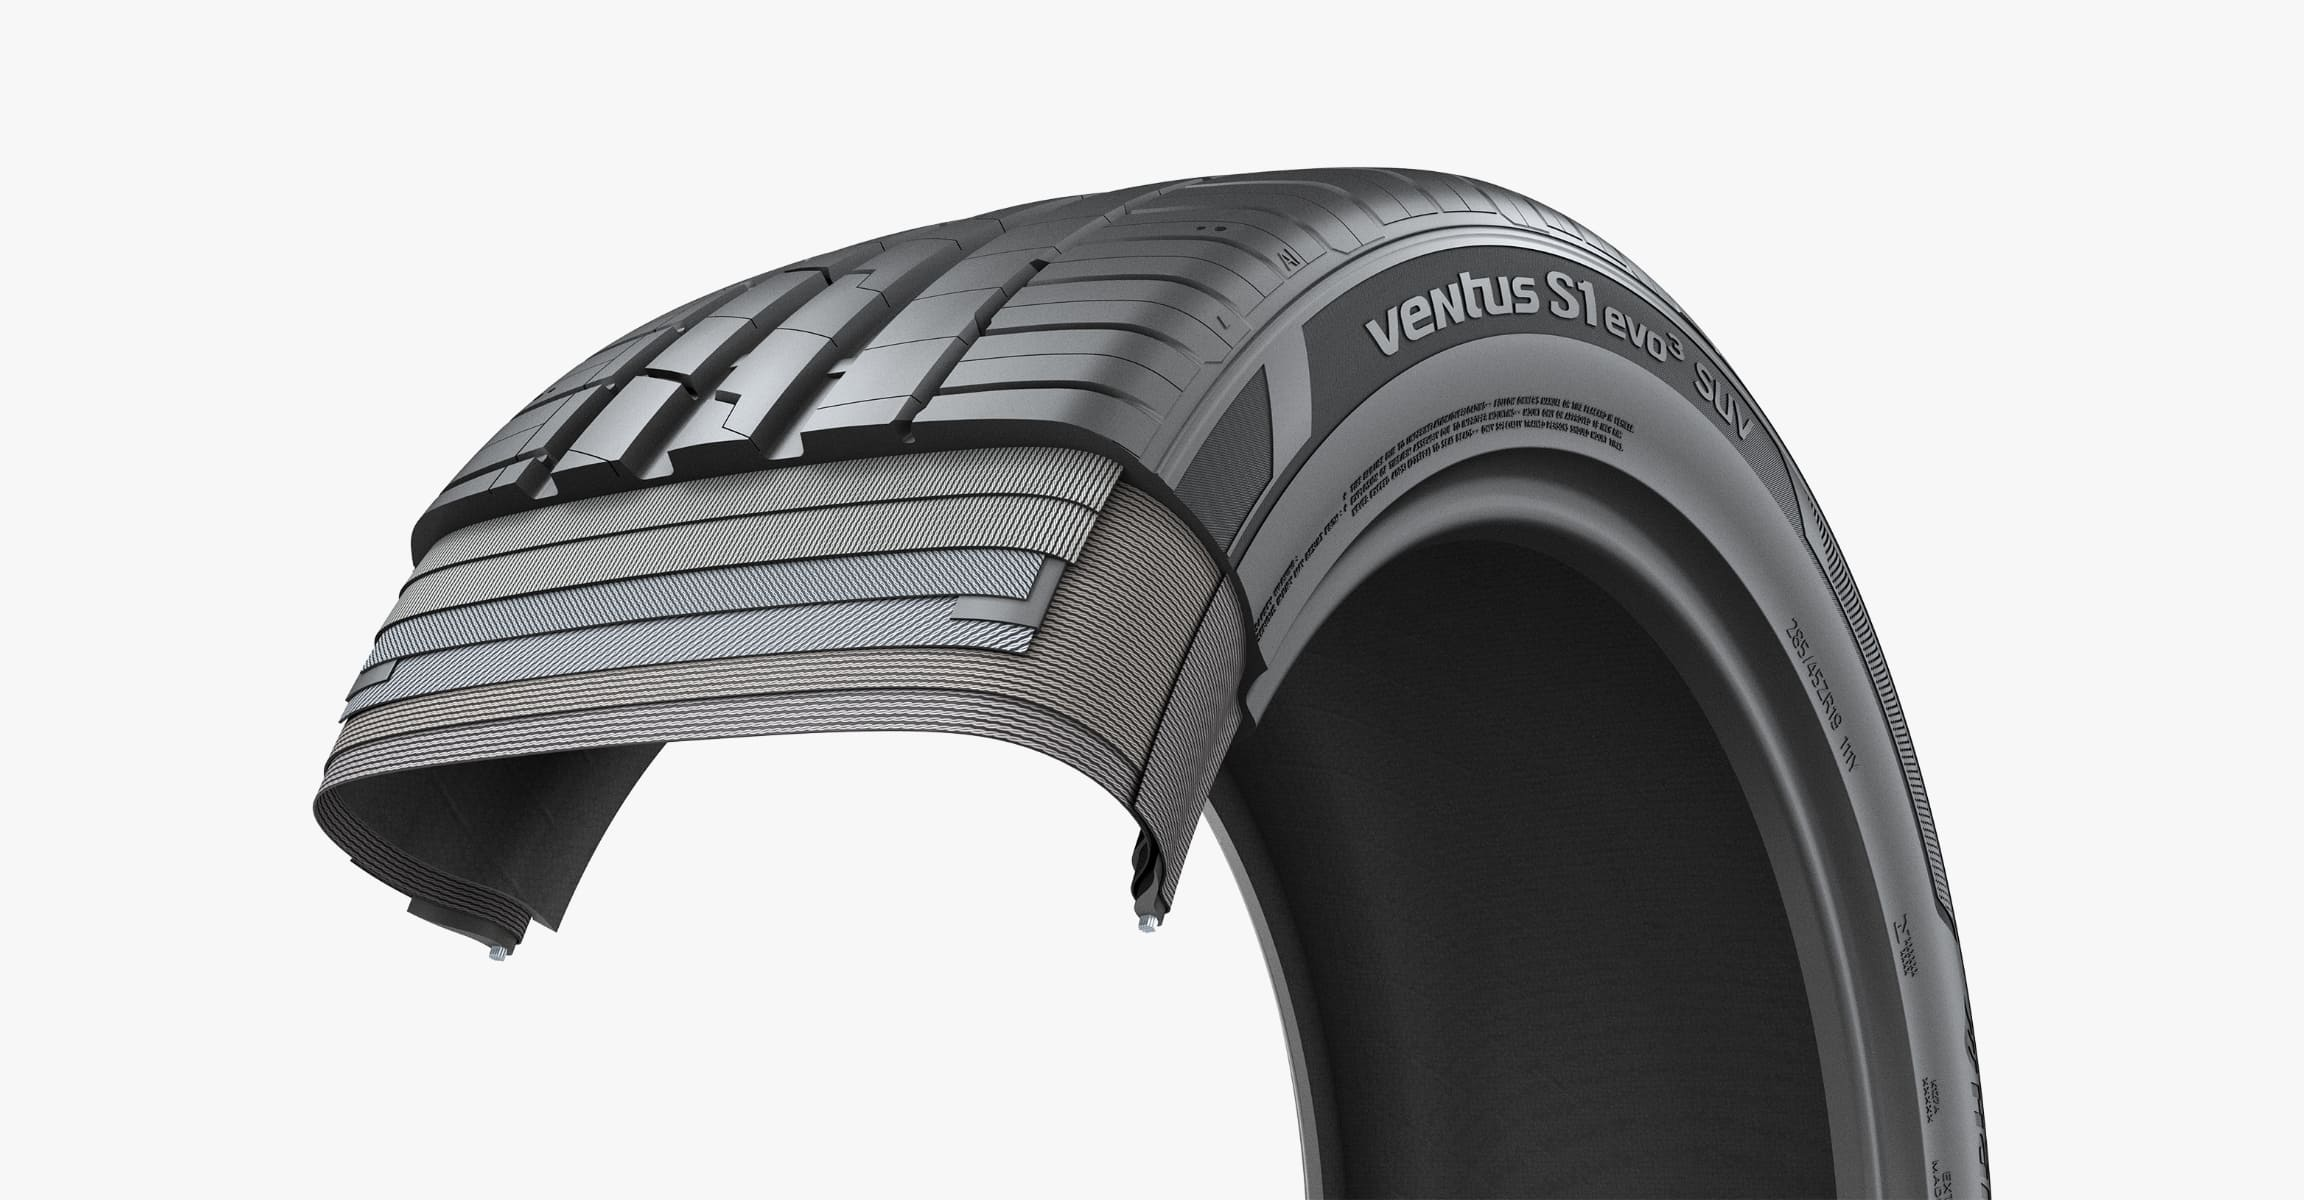
\includegraphics[scale=0.15]{Immagini/Tyres/Tire Structure_w.jpg}
    \caption{Struttura del pneumatico}
    \label{fig:Structure_tyres}
\end{figure}
\begin{description}
    \item[Carcassa :] è la parte più importante perchè rappresenta il telaio dello pneumatico. Il termine carcassa indica tutti gli strati composti dalle nappe a trama dello pneumatico. Assorbe la pressione dell'aria interna allo pneumatico, il peso e i colpi.
    \item [Strato intermedio e cintura :]
    è una struttura a nido d‘ape realizzata con fili di ferro collocata (diagonalmente) tra il battistrada e la carcassa, al fine di proteggere quest'ultima. Assorbe i colpi esterni e impedisce alle scheggiature o alle lesioni al battistrada di venire a diretto contatto con la carcassa. Allo stesso tempo, previene la separazione dello strato di gomma e della carcassa. La cintura ,invece, è un forte strato di rinforzo collocato nella circonferenza tra il battistrada e la carcassa negli pneumatici radiali e cinturati. Le funzioni della cintura sono simili a quelle dello strato intermedio; inoltre, rinforza la solidità del battistrada serrando saldamente la carcassa.
    \item [Spalla :] è la parte di pneumatico collocata tra il battistrada e la parete laterale, essa è composta dallo strato di gomma più spesso dell'intero pneumatico. Ha il compito di garantire la stabilità in curva e mantenere la traiettoria durante la guida.
    \item [Battistrada :] è composto da uno spesso strato di gomma che viene direttamente a contatto con la superficie stradale. È altamente resistente alla rottura e ai colpi, al fine di proteggere la carcassa e la cintura all'interno dello pneumatico. 
    il disegno dello stesso e la mescola di cui è composto sono caratteristica fondamentali che definiscono le prestazioni del pneumatico stesso .
    \item [Parete Laterale :] è collocata tra la spalla e il tallone, ha il compito di proteggere la carcassa e di aumenta le prestazioni di guida attraverso la sua flessibilità.
    \item [Tallone :] Ha il compito di fissare lo pneumatico al cerchione. È formato da varie parti, comprendenti il filo del tallone, il nucleo, la gomma e l'aletta. In generale, il cerchione è leggermente stretto, in modo che, in caso di riduzione improvvisa della pressione dell'aria durante la guida, lo pneumatico non si stacchi improvvisamente dal cerchione.
    \item [Liner interno :]
     consiste in uno strato di gomma con delle qualità ermetiche elevate. La gomma è generalmente composta di butile, da gomma sintetica o da un tipo di poli-isoprene. La funzione principale è quella di mantenere l'aria all'interno dello pneumatico.
\end{description}



\subsubsection{L'effetto del carico verticale}
La pressione media al suolo nell’area di contatto è, in prima approssimazione,
pari alla pressione di gonfiaggio del pneumatico

Il pneumatico, gonfiato ad una pressione p e soggetto ad un carico verticale $F_z$, si deformerà in modo tale da mettere in contatto con il suolo una superficie pari al rapporto $F_z / p$.
Questa deformazione comporterà uno schiacciamento pari ad f.
Più alto è il carico e più bassa è la pressione maggiore sarà la deformazione.

\subsubsection{Caratterizzazione dei pneumatici}
L'analisi del comportamento meccanico dei pneumatici si basa spesso sui risultati ottenuti sperimentalmente su singole gomme.\\
Per caratterizzare il pneumatico rispetto al comportamento direzionale si suppone che la superficie sia perfettamente piana e orizzontale.
Questo tipo di prove sono spesso svolte appoggiando la ruota su un tappeto mobile o su un tamburo rotante con superficie abrasiva.\\
Il sistema consiste in una macchina a disco rotante capace di misurare le forze e i momenti
agenti sullo pneumatico in seguito all’assegnazione di determinati valori di angoli di deriva,
di rollio e carico verticale.\\
Nonostante nessuna di queste prove standard corrisponde alle effettive condizioni di utilizzo i dati ottenuti sono comunque molto utili.
Essi sono di fondamentale importanza poichè nell'ultimo ventennio le simulazioni virtuali di veicoli sono diventate la base per la progettazione e l'ottimizzazione di veicoli.
Questi dati dovrebbero avere un accuratezza abbastanza elevata in modo da garantire una buona attendibilità delle simulazioni, con il passare degli anni sono stati sviluppati modelli empirici sempre più sofisticati in grado di avvicinarsi sempre maggiormente alla realtà.
Tuttavia non sempre i fornitori sono disposti a fornire dati accurati e completi per quanto riguarda i loro prodotti e spesso risultano difficili da reperire.

\subsection{Forze e slip}
Un pneumatico può essere descritto come un sistema in grado di generare forze e momenti come conseguenza degli input applicati.
\begin{figure}[ht]
    \centering
    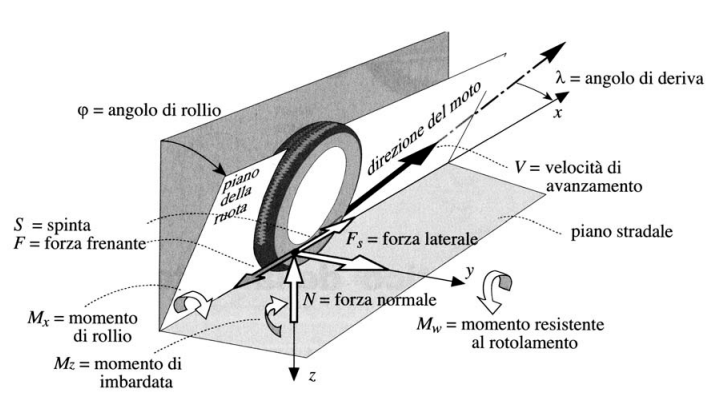
\includegraphics[scale=0.9]{Immagini/Tyres/tyre_forces.png}
    \caption{Forze e momenti generati dallo pneumatico}
    \label{fig:tyre_forces}
\end{figure}
Queste forze e momenti possono essere schematizzati come applicati in corrispondenza del centro del impronta a terra. Essi posso essere riassunti :
\begin{itemize}
    \item Una forza longitudinale, agente lungo la direzione x, assunta positiva in fase di
    accelerazione e negativa in fase di frenata. $\longrightarrow$ [$F_x$]
    \item Una forza laterale, orientata ortogonalmente a quella longitudinale ,direzione y, che garantisce la tenuta del veicolo. $\longrightarrow$ [$F_y$]
    \item Una forza normale al piano della strada, agente in direzione z. $\longrightarrow$ [$F_z$]
    \item Un momento di rollio attorno all’asse x. $\longrightarrow$ [$M_x$]
    \item Un momento di resistenza al rotolamento intorno all’asse y. $\longrightarrow$ [$M_y$]
    \item Un momento di imbardata intorno all’asse z. $\longrightarrow$ [$M_z$] 

\end{itemize}




\subsection{Magic Formula}
La Magic Formula è un modello empirico-matematico creato da Hans Bastiaan Pacejka, che che cerca di riassumere le prestazioni sperimentali dello pneumatico attraverso formule matematiche. Queste hanno una precisa struttura in cui compaiono coefficienti ricavati sperimentalmente e i parametri di funzionamento. L'obbiettivo è fornire in output varie forze e momenti che il pneumatico può generare.\\
La formulazione base è:
\begin{equation}
\label{eq:Pacjeka}
    y(x)=D*sin(C*arctant(Bx-E(Bx-arctan(Bx)))
\end{equation}
In questa formulazione la Y rappresenta la variabile in output desiderata, può essere
$F_x$, $F_y$ oppure $M_z$, $X$è la variabile in input scelta tra $\alpha$ e $k$. I Coefficenti B, C, D, E, chiamati anche coefficienti di Pacejka, esprimono:
\begin{itemize}
    \item B $\longrightarrow$ Stiffness factor \hspace{2.3cm} B $>$ 0
    \item C $\longrightarrow$ Shape factor     \hspace{2.3cm} 1 $<$ C $<$ 2
    \item D $\longrightarrow$ Peak value       \hspace{2.6cm} D $= \mu*F_Z$
    \item E $\longrightarrow$ Curvature factor \hspace{2cm} E $<$ 1
\end{itemize}
I range consigliati sono presi da \cite{Guiggiani}.

\subsection{Evoluzione della Magic Formula}
La prima versione della Magic formula è stata sviluppata nel 1987 da allora sono state create una serie di nuove versioni.
Nel 1996 TNO automotive ha introdotto modello di pneumatico MF-Tyre 5.0 ed il software commerciale MF-Tool per l'identificazione dei parametri. Questi sono basati sulle equazioni presentate nell'articolo di Pacejka del 1996 \cite{Pacejka1997MagicFT}.\\ 
Nel corso degli anni sono stati apportati alcuni miglioramenti (es. aggiunta del
momento di ribaltamento, slittamento combinato migliorato, ecc.) e sono stati rilasciati i modelli: MF-Tyre 5.1 e MF-Tyre 5.2 seguentemente.\\ 
MF-Tyre è stato concepito specificatamente per autovetture e camion utilizzanti pneumatici con
angoli di inclinazione (camber) relativamente piccoli (fino a 10 gradi).\\
È stato necessario modificare le equazioni della MF, creando il modello MF-MCTyre 1.0 per poterlo utilizzare per i pneumatici delle moto che notoriamente lavorano con angoli di inclinazione molto più elevati. In una fase successiva si è migliorata la precedente versione rilasciando il MF-MCTyre 1.1.\\
Nella versione MF-Tyre 6.0 le equazioni sono state ri-adattate, in modo che un unico modello possa gestire sia i pneumatici per le auto che per le moto.
È stato aggiunto inoltre il turn slip per rappresentare, ad esempio, il momento di autoallineamento
che si verifica durante la sterzata del pneumatico a veicolo fermo.\\ 
La MF-Tyre 6.1 estende le equazioni per poter incorporare gli effetti delle variazioni nella pressione di gonfiaggio.\\
La MF-Tyre 6.2 il raggio di carico viene aggiornato per ampi slittamenti laterali e camber
angoli. ed inoltre rende disponibile l'estensione MF-Swift per motociclette. MF-Swift utilizza un modello ad anello rigido cioè si assume che la cintura del pneumatico si comporti come un corpo rigido. Questo comporta un attendibilità maggiore nella gamma di frequenze in cui la flessione della cintura del pneumatico può essere trascurata, a seconda del tipo di pneumatico siamo tra i 60 e i 100 Hz.\\ 
Il modello include gli effetti giroscopici, esso utilizza un singolo punto di contatto per il calcolo dello slittamento. Riesce a descrivere lo slittamento in transitorio, fino allo scorrimento completo, grazie al diminuzione della lunghezza di rilassamento all'aumentare dello slip. \\
MF-Swift è adatto per prove con raggi di curvatura che abbiano lunghezza d'onda dell'ordine di due volte la lunghezza del contatto.\\ 
\begin{figure}[!h]
    \centering
    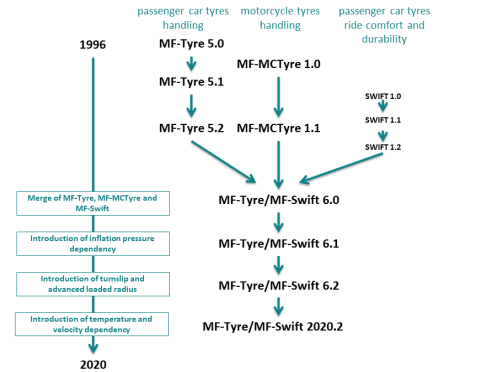
\includegraphics[scale=0.8]{Immagini/Tyres/MF-Tire History.png}
    \caption{}
    \label{fig:MF-Tire version history}
\end{figure}
\\
Per convenzione si utilizza una parola univoca che identifica la versione utilizzata è "FITTYP", questo parametro si trova nella sezione [model] del file.tir

\begin{itemize}
    {\tiny
    \setlength\itemsep{-0.5em}
    \item FITTYP = 5 \hspace{0.33cm} $\longrightarrow$ \hspace{0.2cm} MF-Tyre 5.0 , 5.1
    \item FITTYP = 6 \hspace{0.33cm} $\longrightarrow$ \hspace{0.2cm} MF-Tyre 5.2
    \item FITTYP = 21 \hspace{0.2cm} $\longrightarrow$ \hspace{0.2cm} 
    MF-Swift 1.1  (basato su MF-Tyre 5.2)
    \item FITTYP = 51 \hspace{0.2cm} $\longrightarrow$ \hspace{0.2cm} MF-MCTyre 1.0
    \item FITTYP = 52 \hspace{0.2cm} $\longrightarrow$ \hspace{0.2cm} MF-MCTyre 1.1
    \item FITTYP = 60 \hspace{0.2cm} $\longrightarrow$ \hspace{0.2cm} MF-Tyre 6.0
    \item FITTYP = 61 \hspace{0.2cm} $\longrightarrow$ \hspace{0.2cm} MF-Tyre 6.1
    \item FITTYP = 62 \hspace{0.2cm} $\longrightarrow$ \hspace{0.2cm} MF-Tyre 6.2
    \item FITTYP = 70 \hspace{0.2cm} $\longrightarrow$ \hspace{0.2cm} MF-Tyre 6.2 + Temperature and Velocity model

    }
\end{itemize}

\subsubsection{Tire property file}
Le version MF-Tyre precedentemente elencate sono modelli di simulazione di pneumatici definiti da una serie di parametri. Questi parametri vengono generalmente archiviati in dei file, chiamati "Tire Property File". Questo file ha tipicamente l'estensione ".tir".\\ 
La figura \ref{fig:Structure_file_tir} mostra la classica struttura e il contenuto del file.\\
\begin{figure}[ht]
    \centering
    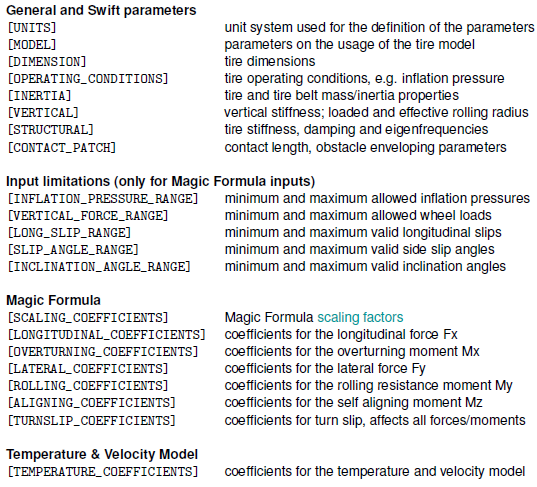
\includegraphics[scale=0.9]{Immagini/Tyres/Structure_file_tir.png}
    \caption{}
    \label{fig:Structure_file_tir}
\end{figure}
Nella prima sezione del file sono elencate tutte le informazioni generali , le unità di misura , tutte le caratteristiche geometriche del pneumatico
e le proprietà strutturali dello stesso.\\
Nella seconda sezione vengono elencati i limiti di pressione , forza verticale , vari slip e camber ai quali il modello può operare.\\
La terza sezione è la più ampia, all'interno si trovano numerosi coefficienti, di seguito elencheremo i più significativi.\\
I coefficienti di scala iniziano con la lettera L essi vengono inclusi nel modello per poter ottenere un modello che simuli la realtà nel modo più affine possibile.
Come visto nell'introduzione ai pneumatici, le prove di forza e momenti vengono spesso eseguite ambiente di laboratorio.\\ 
La superficie stradale artificiale sulla macchina di prova per pneumatici può essere molto diversa rispetto al reale manto stradale.
Combinato all'incertezza sulla temperatura, umidità, usura, pressione di gonfiaggio, ecc. il comportamento del pneumatico montato sul veicolo potrebbe discostarsi in modo significativo rispetto ai risultati ottenuti mediante la macchina di prova.\\
Verosimilmente si potrebbero avere differenze fino al 20$\%$ nel coefficiente di attrito e nella cornering stiffness \cite{Braghin2006EnvironmentalEO}.\\
I più importanti fattori di scala sono:\\
\begin{table}[h!] 
    {\scriptsize\setlength\itemsep{-0.2em}
    \centering
    \begin{tabular}{l l}
        \texttt{LMUX} \qquad \quad  & Scale factor of longitudinal peak friction coefficient\\
        \texttt{LKX} & Scale factor of longitudinal slip stiffness\\
        \texttt{LMUY} & Scale factor of lateral peak friction coefficient cornering stiffness\\
        \texttt{LKY} & Scale factor of cornering stiffness\\
        \texttt{LKYC} & Scale factor of camber stiffness\\
        \texttt{LTR} & Scale factor of pneumatic trail\\
        \texttt{LKZC} & Scale factor of camber moment stiffness\\
        \texttt{LMP} & Scale factor of parking moment at standstill\\
    \end{tabular}

    }
    \caption{}
    \label{tab:scaling factors}
\end{table}
\\
I coefficienti della sezione 3 verranno discussi 
approfonditamente nelle successive sottosezioni.\\
La quarta sezione contiene i coefficienti per gli effetti termici e gli effetti di velocità.
Tuttavia essa si trova molto raramente per via della complessità che accompagna questi effetti.

\subsubsection{MF 5.2}
Fin dalla sua concezione, oltre 20 anni fa, la Magic Formula è stata adottata abbastanza rapidamente nell' industria come modello di pneumatico standard per simulazioni di manovrabilità dei veicoli.\\ 
Nel corso degli anni sono stati apportati vari sviluppi
migliorare l'accuratezza ed estendere le capacità del modello, ad esempio il metodo per descrivere lo slip combinato è stato migliorato.\\
Il modello di pneumatico MF-Tire 5.2 ha dimostrato una buona attendibilità ed è tuttora ampiamente utilizzato negli studi dinamica dei veicoli. 
Le equazioni del modello \\


\subsubsection{MF 6.1}
Il modello MF-Tire 5.2 necessitava di alcune evoluzioni che ne ampliassero le potenzialità,
gli obbiettivi erano:\\
-Migliorare la descrizione del camber, attraverso una formulazione e un un controllo espliciti sulla rigidità al camber ed estendere le capacità del modello nel gestire angoli molto ampi (motocicli).\\
-Includere l'effetto della pressione di gonfiaggio. Questo permetteva di eliminare i diversi file per diverse pressioni dei pneumatici in quanto consente di prevedere 
comportamento anche a pressioni differenti rispetto a quello con il quale si è svolta il test sperimentale, riducendo di conseguenza il numero di misurazioni richieste.
-Rendere coerente la descrizione della dinamica dei pneumatici tra MF-Swift e MF-Tire. Includendo l'effetto della carcassa e del rilassamento del pneumatico 
Inoltre sono stati apportati ulteriori miglioramenti, ad esempio nella descrizione della resistenza al rotolamento e del momento di ribaltamento.
Tutto ciò è stato implementato attraverso la versione 6.1 (MF-Tyre 6.1).\\

\begin{figure}[ht]
    \centering
    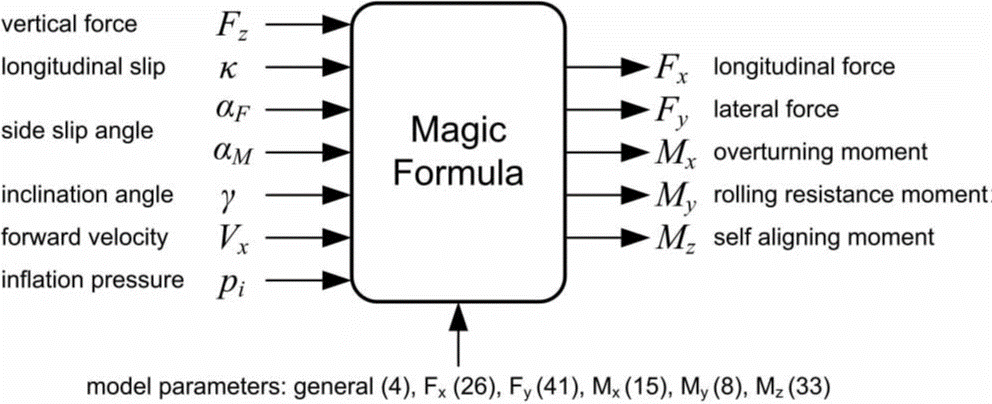
\includegraphics[scale=0.6]{Immagini/Tyres/MF.png}
    \caption{Input e output del modello MF-6.1}
    \label{fig:MF_tyres}
\end{figure}

\begin{figure}[ht]
    \centering
    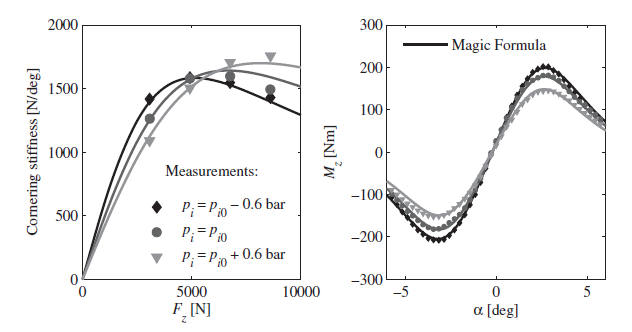
\includegraphics[scale=0.8]{Immagini/Tyres/Tyre pressure effects for a passenger car tyre.png}
    \caption{Effetto della pressione di gonfiaggio sulla cornering stiffness e sul momento di autollineamento}
    \label{fig:Pressure effects}
\end{figure}

La fig. \ref{fig:Pressure effects} mostra come al diminuire della pressione di gonfiaggio, la cornering stiffness aumenti in modo più rapido al crescere di $F_Z$ fino a valori di 5000[N] questo è dovuto al fatto .............\\

\begin{figure}[ht]
    \centering
    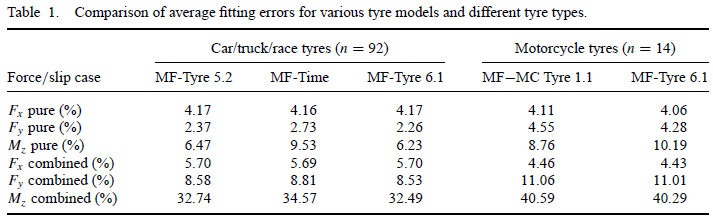
\includegraphics[scale=0.8]{Immagini/Tyres/comparison MF-Tire version.png}
    \caption{Confronto fra le versioni MF-Tire}
    \label{fig:Comparison MF-Tire version}
\end{figure}
 

I Grafici riportati sono presi da \cite{Besselink2010AnIM}.\\

\section{Dinamica Laterale}
La fonte di questo argomento è ....., mentre ulteriori approfondimenti si trovano in 
In questo capitolo verranno descritte le basi della dinamica del veicolo per quanto concerne la dinamica laterale.
\\Per l'analisi (quasi)-stazionaria verranno utilizzati semplici modelli di veicoli. 
Verranno introdotte le caratteristiche della forza laterale effettiva sui pneumatici........ 




\subsection{Single track model}
è il modello più semplice utilizzato per analizzare le dinamiche laterali dei veicoli
\subsection{Double track model}
\subsubsection{Trasferimento di carico laterale}
\subsubsection{Ackermann steering}
\subsubsection{Camber}
\subsubsection{Aerodinamica}
